\chapterimage{MathCover.png}
\chapter{Water Math - Week 3}



\begin{table}[H]
\begin{tabular}{| m{1cm} | m{1cm} | m{12cm} |}
\hline
\multicolumn{3}{|l|}{\textbf{Expected   Range of Knowledge for Math}}                                                                      \\ \hline
\multicolumn{3}{|l|}{\textit{Water   Distribution System Operator License Exams}}                                                          \\ \hline
\multicolumn{1}{l|}{} & \multicolumn{1}{l|}{D1-D5} & Ability to calculate   flow rates for a storage facility                     \\ \cline{2-3} 
\multicolumn{1}{l|}{} & \multicolumn{1}{l|}{D1-D5} & Ability to calculate   the volume of a storage facility                      \\ \cline{2-3} 
\multicolumn{1}{l|}{} & \multicolumn{1}{l|}{D1-D5} & Knowledge of unit   conversions                                              \\ \cline{2-3} 
\multicolumn{1}{l|}{} & \multicolumn{1}{l|}{D1-D5} & Ability to calculate   flow rates                                            \\ \cline{2-3} 
\multicolumn{1}{l|}{} & \multicolumn{1}{l|}{D1-D5} & Ability to calculate   pipe volumes                                          \\ \cline{2-3} 
\multicolumn{1}{l|}{} & \multicolumn{1}{l|}{D1-D5} & Ability to calculate   the area of a pipe cross-section                      \\ \cline{2-3}
\multicolumn{1}{l|}{} & \multicolumn{1}{l|}{D1-D5} & Ability to calculate   the volume of a trench                                \\ \cline{2-3}  
\multicolumn{1}{l|}{} & \multicolumn{1}{l|}{D1-D5} & Ability to calculate   the surface area of a valve face                      \\ \cline{2-3} 
\multicolumn{1}{l|}{} & \multicolumn{1}{l|}{D1-D5} & Ability to calculate   the volume of a cylinder, rectangle, and square       \\ \cline{2-3} 
\multicolumn{1}{l|}{} & \multicolumn{1}{l|}{D1-D5} & Ability to calculate   the volume of a pipe                                  \\ \cline{2-3} 
\multicolumn{1}{l|}{} & \multicolumn{1}{l|}{D1-D5} & Ability to calculate   the volume of a well, storage reservoir, pipe, trench \\ \cline{2-3} 
\multicolumn{1}{l|}{} & \multicolumn{1}{l|}{D1-D5} & Ability to calculate   the well draw down                                    \\ \cline{2-3} 
\multicolumn{1}{l|}{} & \multicolumn{1}{l|}{D1-D5} & Ability to calculate   total force on a valve                                \\ \cline{2-3} 
\multicolumn{1}{l|}{} & \multicolumn{1}{l|}{D1-D5} & Ability to convert   pressure to feet of head                                \\ \cline{2-3} 
\multicolumn{1}{l|}{} & \multicolumn{1}{l|}{D1-D5} & Ability to convert   units of volume, area, and time                         \\ \cline{2-3} 
\multicolumn{1}{l|}{} & \multicolumn{1}{l|}{D1-D5} & Ability to convert   units of volume, area, pressure, and time               \\ \cline{2-3} 
\multicolumn{1}{l|}{} & \multicolumn{1}{l|}{D1-D5} & Ability to convert   units of volume, pressure and area                      \\ \cline{2-3} 
\multicolumn{1}{l|}{} & \multicolumn{1}{l|}{D1-D5} & Ability to convert   water units                                             \\ \cline{2-3} 
\multicolumn{1}{l|}{} & \multicolumn{1}{l|}{D2-D5} & Ability to calculate   pipe capacity                                         \\ \cline{2-3} 
\multicolumn{1}{l|}{} & \multicolumn{1}{l|}{D2-D5} & Ability to calculate   the velocity of water                                 \\ \cline{2-3} 
\multicolumn{1}{l|}{} & \multicolumn{1}{l|}{D2-D5} & Ability to calculate   thrust block size                                     \\ \cline{2-3} 
\multicolumn{1}{l|}{} & \multicolumn{1}{l|}{D2-D5} & Ability to convert a   pressure reading to depth of water                    \\ \cline{2-3} 
\multicolumn{1}{l|}{} & \multicolumn{1}{l|}{D2-D5} & Ability to convert a   scale to actual distance                              \\ \cline{2-3} 
\end{tabular}
\end{table}
\newpage






\begin{table}[H]
\begin{tabular}{| m{1cm} | m{1cm} | m{12cm} |}
\hline
\multicolumn{3}{|l|}{\textbf{Expected   Range of Knowledge for Math}}                                                                      \\ \hline
\multicolumn{3}{|l|}{\textit{Water   Distribution System Operator License Exams (Continued)}}                                                          \\ \hline
\multicolumn{1}{l|}{} & \multicolumn{1}{l|}{D3-D5} & Ability to calculate   brake-horsepower                                      \\ \cline{2-3} 
\multicolumn{1}{l|}{} & \multicolumn{1}{l|}{D3-D5} & Ability to calculate   pump efficiency                                       \\ \cline{2-3} 
\multicolumn{1}{l|}{} & \multicolumn{1}{l|}{D3-D5} & Ability to calculate   specific yield of a well                              \\ \cline{2-3} 
\multicolumn{1}{l|}{} & \multicolumn{1}{l|}{D3-D5} & Ability to calculate   the cost of water production                          \\ \cline{2-3} 
\multicolumn{1}{l|}{} & \multicolumn{1}{l|}{D4-D5} & Ability to calculate a water loss rate                                       \\ \cline{2-3} 
\multicolumn{1}{l|}{} & \multicolumn{1}{l|}{D4-D5} & Ability to calculate the cost of pumping   water                             \\ \cline{2-3} 
\multicolumn{1}{l|}{} & \multicolumn{1}{l|}{D4-D5} & Ability to calculate the hydraulic gradient                                  \\ \cline{2-3} 
\multicolumn{1}{l|}{} & \multicolumn{1}{l|}{D4-D5} & Ability to calculate water production costs                                  \\ \hline
\multicolumn{3}{|l|}{Water   Treatment Operator License Exams}                                                                    \\ \hline
\multicolumn{1}{l|}{} & \multicolumn{1}{l|}{T1-T4} & Ability to calculate   flow rates and water velocity                         \\ \cline{2-3} 
\multicolumn{1}{l|}{} & \multicolumn{1}{l|}{T1-T4} & Ability to calculate   the volume of water in a storage facility             \\ \cline{2-3} 
\multicolumn{1}{l|}{} & \multicolumn{1}{l|}{T1-T4} & Ability to calculate   well head pressure                                    \\ \cline{2-3} 
\multicolumn{1}{l|}{} & \multicolumn{1}{l|}{T1-T4} & Ability to convert   common water units (e.g. gallons per minute to MGD)     \\ \cline{2-3} 
\multicolumn{1}{l|}{} & \multicolumn{1}{l|}{T1-T4} & Ability to convert   head pressure to water elevation                        \\ \cline{2-3} 
\multicolumn{1}{l|}{} & \multicolumn{1}{l|}{T1-T4} & Ability to convert   units of length, volume, flow and pressure              \\ \cline{2-3} 
\multicolumn{1}{l|}{} & \multicolumn{1}{l|}{T1-T4} & Ability to determine   water level in a storage tank, reservoir, or well     \\ \cline{2-3} 
\multicolumn{1}{l|}{} & \multicolumn{1}{l|}{T1-T4} & Ability to calculate   a chemical dosage                                     \\ \cline{2-3} 
\multicolumn{1}{l|}{} & \multicolumn{1}{l|}{T1-T4} & Ability to calculate   a chemical solution concentration                     \\ \cline{2-3} 
\multicolumn{1}{l|}{} & \multicolumn{1}{l|}{T1-T4} & Ability to calculate   chlorine demand and chlorine residual                 \\ \cline{2-3} 
\multicolumn{1}{l|}{} & \multicolumn{1}{l|}{T1-T4} & Ability to convert   common water units, (gallons per minute to MGD, etc...) \\ \cline{2-3} 
\multicolumn{1}{l|}{} & \multicolumn{1}{l|}{T1-T4} & Ability to determine   water level in a storage tank, reservoir or well      \\ \cline{2-3} 
\multicolumn{1}{l|}{} & \multicolumn{1}{l|}{T3-T4} & Ability to perform   blending calculations                                   \\ \cline{2-3} 
\multicolumn{1}{l|}{} & \multicolumn{1}{l|}{T3-T4} & Ability to calculate   a dilution factor                                     \\ \cline{2-3} 
\multicolumn{1}{l|}{} & \multicolumn{1}{l|}{T3-T4} & Ability to mix   chemicals and prepare reagents                              \\ \cline{2-3} 
\multicolumn{1}{l|}{} & \multicolumn{1}{l|}{T3-T4} & Ability to perform   dilutions                                               \\ \cline{2-3} 
\multicolumn{1}{l|}{} & \multicolumn{1}{l|}{T3-T4} & Ability to calculate   a coagulant dose from a jar test                      \\ \cline{2-3} 
\multicolumn{1}{l|}{} & \multicolumn{1}{l|}{T3-T4} & Ability to calculate   a filter-aid dosage                                   \\ \cline{2-3} 
\multicolumn{1}{l|}{} & \multicolumn{1}{l|}{T3-T4} & Ability to calculate   a filtration rate                                     \\ \cline{2-3} 
\multicolumn{1}{l|}{} & \multicolumn{1}{l|}{T3-T4} & Ability to calculate   filter loading rate                                   \\ \cline{2-3} 
\multicolumn{1}{l|}{} & \multicolumn{1}{l|}{T3-T4} & Ability to calculate   percent or log removal of contaminants from water     \\ \cline{2-3} 
\multicolumn{1}{l|}{} & \multicolumn{1}{l|}{T3-T4} & Ability to calculate   the cost of water treatment operations                \\ \cline{2-3} 
\end{tabular}
\end{table}
\newpage



\section{Ratio and Proportion}\index{Ratio and Proportion}
\textbf{Ratio:}\\
\begin{itemize}
\item Ratio is used for comparing the size of two or more quantities.
\item Say if there are 10 red cubes and 5 pink marbles in a bag, the ratio $\dfrac{5}{10}$ is the ratio of pink marbles and red cubes.  It can also be represented by 5:10.
\item 5 lbs of chemical in 10 gallons solution is a ratio.  So is 30 miles per gallon.
\item Unlike fractions, ratio does not compare things that have the same units.
\end{itemize}
\textbf{Proportion:}\\
\begin{itemize}
\item Two quantities are said to be in proportion if one changes, the other changes in a specific way.
\item Two quantities are said to be directly proportional, if the \textbf{increase} in one will \textbf{increase} the other value proportionally.  
\begin{itemize}
\item Thus, if two quantities x and y are directly proportional, its ratio $\dfrac{x}{y}$ will be a fixed value. Thus for x$_1$ and y$_1$ different values of x and y respectively will be related by the equation $\dfrac{x}{y}=\dfrac{x_1}{y_1}$.  

\item This relationship is useful for calculating unknown values in water treatment calculations as in the following example: \\
\vspace{0.2cm}
Knowing 200 lbs of bleach is needed to disinfect 5 MG of water at a treatment plant, calculate the lbs of bleach required to disinfect 3.2 MGD flow.\\

\vspace{0.2cm}

The ratio $\dfrac{200 \enspace pounds \enspace bleach}{5 MG}$ or 40 lbs bleach per MG is a constant.  
Using this known proportion the lbs of bleach is needed to disinfect 3.2 MG at this plant can be calculated as follows by setting up the equation as:\\
\vspace{0.2cm}
$\dfrac{40 \enspace pounds \enspace bleach}{MG}=\dfrac{X}{3.2 \enspace MG}$ where X is the unknown lbs of bleach that is required to disinfect the 3.2 MG flow.\\
\vspace{0.2cm}
X can be calculated by cross multiplying the above equation: $X=\dfrac{3.2*40}{1}=128 \enspace lbs \enspace bleach$
\end{itemize}
\item Two quantities are said to be inversely proportional if the \textbf{increase} in one will \textbf{decrease} the other value proportionally.  
\begin{itemize}
\item Thus, if two quantities x and y are inversely proportional, its product $x * \text{y}$ will be a fixed value and different values of x and y respectively will be related by the equation $x *y = x_1 * y_1$.
\item Examples of inversely proportional relationship include:\\
\vspace{0.2cm}
\begin{itemize}
\item Labor hours required to perform a certain task or time required to pump down a wetwell depending on the size of the pump.  An increase in assignment of labor hours will reduce the time required to perform the task 
\item Using a larger pump will reduce the time to pump down the wetwell.  
\item In the Pounds formula:\\
\vspace{0.2cm}
$$lbs \enspace \textbf{or} \enspace \dfrac{lbs}{day}=Concentration\Big(\dfrac{mg}{l}\Big)*8.34*volume(MG) \enspace \textbf{or} \enspace Flow (MGD)$$\\
 
\vspace{0.2cm}

for the same lbs or lbs/day, concentration varies inversely with volume or flow.  Thus, for a certain pounds added, the concentration will go down if the flow increases and vice versa.
\item In the flow equation, Q=V*A, for the same flow (Q), velocity (V) and surface area (A) are inversely related.  If Q is remaining the same, an increase in surface area will reduce the velocity and vice versa.\\

Additionally, for a flow through a pipe as the surface area of the pipe is proportional to the square of the diameter, the velocity in the pipe is inversely proportional to the square of the diameter.\\

\vspace{0.2cm}

For a constant Q:  $V *A = V_1 *A_1$ or $V *D^2 = V_1 *D_1^2$

\end{itemize}
\vspace{0.2cm}


\vspace{0.2cm}

\item Application of inversely proportional relationship in water related calculation can be demonstration with the following example:

If it takes 20 minutes to pump a wet well down with one pump pumping at 125 gpm, then how long will it take if a 200 gpm pump is used?

As this is an inversely proportional relationship ( a larger pump will reduce the time required):\\
\vspace{0.2cm}
$(20 \mathrm{minutes} * 125 \mathrm{gpm})=(X \mathrm{minutes} * 200 \mathrm{gpm})$ \\

where X is the unknown time to pump down the wetwell with the 200 gpm pump.\\
\vspace{0.2cm}
Solving for X: $X=\dfrac{20*125}{200}=12.5 \enspace \mathrm{minutes}$
\end{itemize}
\end{itemize}


% \begin{tcolorbox}[breakable, enhanced,
% colframe=blue!25,
% colback=blue!10,
% coltitle=blue!20!black,  
% title= Practice Problems]

% \begin{enumerate}
% \item It takes 6 gallons of chlorine solution to obtain a proper residual when the flow is 45,000 gpd. How many gallons will it take when the flow is 62,000 gpd?

% \item A motor is rated at 41 amps average draw per leg at $30 \mathrm{Hp}$. What is the actual $\mathrm{Hp}$ when the draw is 36 amps? C. 

% \item If it takes 2 operators $4.5$ days to clean an aeration basin, how long will it take three operators to do the same job?

% \item It takes 3 hours to clean 400 feet of collection system using a sewer ball. How long will it take to clean 250 feet?

% \item It takes 14 cups of $\mathrm{HTH}$ to make a $12 \%$ solution, and each cup holds 300 grams. How many cups will it take to make a $5 \%$ solution?

% \item A bike travelling at 5 miles/hr completes a journey in 40 minutes. How long would the same journey take if the speed was increased to 8 miles/hr?
% \end{enumerate}
% \end{tcolorbox}








\newpage

\section{Unit Conversions}\index{Unit Conversions}
\begin{itemize}
\item A conversion is a number that is used to multiply or divide into a measure in order to change the units of the original measure.

\begin{table}[h!]

\begin{center}
    \begin{tabular}{ | p{4cm} |p{8cm}|}
    \hline
    
\textbf{Measure} & \textbf{Units}\\
\hline   
Length  & inches, ft, miles\\
\hline 
Area  & ft$^2$, acres \\
\hline 
Volume & ft$^3$, gallons, acres-ft.\\
\hline 
Density & weight per volume, lbs/ft$^3$, lbs/gallon\\
\hline 
Flow & ft$^3$/min, MGD, acres-ft/day\\
\hline 

	

    \end{tabular}
 \caption{Common units in water calculations}	
    \end{center}

    \end{table}

\item In most instances, the conversion factor cannot be derived. It must be known. Therefore, tables such as the one below are used to find the common conversions.\\
\begin{tabular}{|l|l|}
\hline
Some Common Conversions & Weight \\
\hline
Linear Measurements & $1 \mathrm{ft}^{3}$ of water $=62.4 \mathrm{lbs}$ \\
\hline
1 inch $=2.54 \mathrm{~cm}$ & $1 \mathrm{gal}=8.34 \mathrm{lbs}$ \\
$1 \mathrm{foot}=30.5 \mathrm{~cm}$ & $1 \mathrm{lb}=453.6 \mathrm{grams}$ \\
$1 \mathrm{~meter}=100 \mathrm{~cm}=3.281 \mathrm{feet}=39.4$ inches 1 & $1 \mathrm{~kg}=1000 \mathrm{~g}=2.2 \mathrm{lbs}$ \\
acre $=43,560 \mathrm{ft}^{2}$ & $1 \%=10,000 \mathrm{mg} / \mathrm{L}$ \\
$1 \mathrm{yard}=3 \mathrm{feet}$ & $1 \mathrm{pound}=16 \mathrm{oz} \mathrm{dry} \mathrm{wt}$ \\
 & $1 \mathrm{ft}^{3}=62.4 \mathrm{lbs}$ \\
\hline
Volume & Pressure \\
\hline
$1 \mathrm{gal}=3.78$ liters & $1 \mathrm{ft}$ of head $=0.433 \mathrm{psi}$ \\
$1 \mathrm{ft}=7.48$ gal & $1 \mathrm{psi}=2.31 \mathrm{ft}$ of head \\
$1 \mathrm{~L}=1000 \mathrm{~mL}$ &  \\
$1 \mathrm{gal}=16 \mathrm{cups}$ &  \\
\hline
Flow &  \\
\hline
$1 \mathrm{cfs}=448 \mathrm{gpm}$ &  \\
$1 \mathrm{gpm}=1440 \mathrm{gpd}$ &  \\
\hline
\end{tabular}
\vspace{0.2cm}
\item Common conversions in water related calculations include the following:

\begin{itemize}
  \item gpm to cfs

  \item Million gallons to acre feet

  \item Cubic feet to acre feet

  \item Cubic feet of water to gallons


  \item gpm to MGD 

  \item psi to feet of head

\end{itemize}

\item Steps for unit conversion:\\
\begin{enumerate}[Step 1:]
\item \texthl{Make sure the original unit is for the same measurement as the converted (desired) unit.}  So if the original unit is for area, say in ft$^2$ the converted unit should be another area unit such as in$^2$ or acre but it cannot be gallons as gallon is a unit of volume.\\
Note:  Calculating the weight of a certain volume of water involves the use of density which is the mass per volume -  value in units including lbs/gallon or lbs/$ft^3$\\

\item Write down the conversion formula as:\\

$Quantity \enspace in \enspace converted \enspace unit = Quantity \enspace (\cancel{Original \enspace Unit}) *   Conversion  \enspace Factor \enspace  \dfrac{Conversion \enspace unit}{\cancel{Original \enspace unit}}$\\
\end{enumerate}

\item Note:  If you wish to convert cubic feet of water to pounds, you have to use its density which is the known mass per unit volume.\\
$\dfrac{8.34 \enspace lbs}{gallon}$ or $\dfrac{62.4 \enspace lbs}{ft^3}$\\
$mass \enspace of \enspace water = \cancel{Volume} *   Density  (\dfrac{mass}{\cancel{Volume}})$\\

\end{itemize}

Example Problems:\\
\begin{enumerate}
\item Convert 1000 $ft^3$ to cu. yards\\

$1000 \cancel{ft^3}*\dfrac{cu.yards}{27\cancel{ft^3}} = 37 cu.yards$

\item Convert 10 gallons/min to $ft^3$/hr\\
Note:  This involves use of two conversion factors - one for converting gallons to cubic feet and another for converting minute to gallons.\\ 
$\dfrac{10 \cancel{gallons}}{\cancel{min}}*  \dfrac{ft^3}{7.48 \cancel{gallons}}  * \dfrac{60 \cancel{min}}{hr}   = \dfrac{80.2ft^3}{hr}$


\item Convert 100,000 $ft^3$ to acre-ft.\\
$100,000 \cancel{ft^3} * \dfrac{acre-ft}{43,560 \cancel{ft^2-ft}} =  2.3 acre-ft$\\

\item Convert 8 $ft^3$ of water to pounds.\\
Here the conversion is from a volume ($ft^3$) to a weight (lbs).  It involves use of a standard correlation of the volume of water to its weight - its density. 

$Weight \enspace of \enspace water \enspace in \enspace lbs=8 \cancel{ft^3} *   62.4  (\dfrac{lbs}{\cancel{ft^3}}) = 499.2 \enspace lbs $\\

\end{enumerate}

\subsection{Temperature Conversion}\index{Temperature Conversion}
\begin{itemize}
\item Two scales are commonly used to measure temperature: degrees Fahrenheit (\degree{F}) and degrees Centigrade or Celsius(\degree{C}). 
\item Fahrenheit is the standard scale used in the U.S. and Celsius is the metric scale. 
\item In the Celsius scale, water freezes at 0\degree{C} and boils at 100\degree{C}. In the Fahrenheit scale, water freezes at32\degree{F} and boils at 212\degree{F}. 
\item The following factors can be used when converting from one temperature scale to another:
$$\degree{C} = \dfrac{\degree{F}-32}{1.8}$$

$$\degree{F}=(\degree{C} \times 1.8)+32$$
\end{itemize}

% \newpage

% \begin{tcolorbox}[breakable, enhanced,
% colframe=blue!25,
% colback=blue!10,
% coltitle=blue!20!black,  
% title= Practice Problems]

% \begin{enumerate}
% \item Convert 1000 $ft^3$ to cu. yards\\

% \item Convert 10 gallons/min to $ft^3$/hr\\

% \item Convert 100,000 $ft^3$ to acre-ft.\\

% \item Find the flow in gpm when the total flow for the day is 65,000 gpd.

% \item Find the flow in gpm when the flow is $1.3 \mathrm{cfs}$.

% \item Find the flow in gpm when the flow is $0.25 \mathrm{cfs}$.

% \item The flow rate through a filter is 4.25 MGD. What is this flow rate expressed as gpm?\\

% \item After calibrating a chemical feed pump, you've determined that the maximum feed rate is $178 \mathrm{~mL} /$ minute. If this pump ran continuously, how many gallons will it pump in a full day?

% \item A plant produces 2,000 cubic foot of water per hour. How many gallons of water is produced in an 8-hour shift?

% \item Change 70 °F to °C
% \item Change 140 °F to °C
% \item Change 20 °C to °F
% \item Change 85 °C to °F
% \item Change 4 °C to °F
% \end{enumerate}
% \end{tcolorbox}










\section{Well Hydraulics Calculations} \index{Well Hydraulics Calculations}

\begin{center}
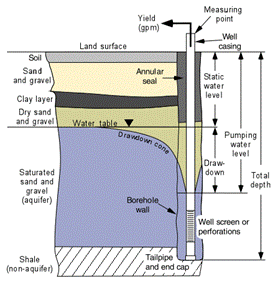
\includegraphics[scale=0.5]{Well1} \hspace{1cm} 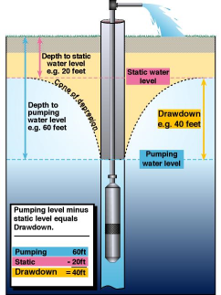
\includegraphics[scale=0.6]{WellDrawdownCalc}
\end{center}

The amount of water a well will produce depends mainly on the type of aquifer, well construction, and the depth of the zone of saturation. The annual recharge rate from percolation, along with the ability of the water bearing formation to transmit water to any given point, will also influence well production. The performance of a well can be determined by taking readings of the hydraulic conditions. An operator must be familiar with these terms and definitions*, in order to accurately troubleshoot problems that may be discovered.\\
\vspace{0.3cm}
\textbf{Static level }is the water level in a well when the pump is not operating.\\
\vspace{0.3cm}
\textbf{Pumping level} is the water level in the well when it is producing.\\
\vspace{0.3cm}
\textbf{Drawdown} is the difference in elevations between the static level and the pumping level. The amount of water produced is approximately proportional to the draw-down. For example, increasing the yield by 10\% will increase the drawdown by 10\%. The draw-down that occurs when a well is running is roughly equal to the head loss encountered in moving the water into the well. Water bearing formations of gravel, limestone and course sand will usually provide more water with less draw-down than formations containing fine sand or clay.\\
\vspace{0.3cm}
\textbf{Specific capacity} is the relationship between the yield of a well and the amount of drawdown in the well. It can be expressed as a ratio of the yield, in terms of gallons per minute, to the drawdown in feet. A well producing 100 gpm with a drawdown of 20 feet would have a specific capacity of 5 gpm per foot of draw-down. In this particular case every time the yield is increased by 5 gpm the drawdown will increase by one foot. This relationship will exist until the yield exceeds the aquifer’s ability to deliver water to any single point, When this limit is reached, the draw-down increases dramatically with little or no increase in the yield.\\
\vspace{0.3cm}
\textbf{Cone of depression} is directly related to the drawdown in the well. As the pump draws down the water level, a portion of the aquifer surrounding the well is drained of water. A cone shaped depression is formed in the water table around the well. The shape of the cone will vary depending on the type of formation in which the well is located. A fine sand formation will usually create a steep cone of depression, while a shallow cone is usually found in coarse sand and gravel formations.\\
\vspace{0.3cm}
\textbf{Radius of influence} is the farthest distance from the well that the cone of depression affects the water table. This distance can be determined by sinking test holes around the well and monitoring the water levels in them while the well is pumping.\\
\vspace{0.3cm}
\textbf{Recovery time} is the amount of time required for the aquifer to stabilize at its static water level once pumping has stopped. This can also be determined by monitoring the water levels in the test holes used to determine the radius of influence.\\
\vspace{0.5cm}
Example Problems:\\
\vspace{0.2cm}
\textbf{Example Problem \#1:} A well is drilled through an unconfined aquifer. The top of the aquifer is 80 feet below grade. After the well was in service for a year, the water level in the well stabilized at 110 feet below grade. What is the drawdown?\\
$\text {Drawdown} =\text { Static Level}-\text { Pumping Level } =80 \mathrm{ft}-110 \mathrm{ft}=30 \mathrm{feet}$
\vspace{0.2cm}
\textbf{Example Problem \#2:} A well produces 300 gpm. If the drawdown is 30 feet, find the specific yield.\\
$\text { Specific Yield } =\dfrac{\text { Yield }}{\text { Drawdown }} =\dfrac{300 \mathrm{gpm}}{30 \mathrm{ft}} =10 \mathrm{gpm} / \mathrm{ft}$\\
  \vspace{0.3cm}
\textbf{Example Problem \#3:} The specific yield for a well is $10 \mathrm{gpm} / \mathrm{ft}$. If the well produces $550 \mathrm{gpm}$, what is the drawdown?\\
  \vspace{0.3cm}
$\text {Specific Yield }=\dfrac{\text { Yield }}{\text { Drawdown }}\implies 10 \mathrm{gpm} / \mathrm{ft}=\dfrac{550 \mathrm{gpm}}{\text { Drawdown }} \implies \text {Drawdown }= \dfrac{550}{10}=\boxed{55 \mathrm{ft}}$ \\
\vspace{0.3cm}
\textbf{Example Problem \#4:} The pumped water level of a well is 400 feet below the surface. The well produces 350 gpm. If the aquifer level is 250 feet below the surface, what is the specific yield for the well?\\
  $\text {Drawdown} =\text { Static Level}-\text { Pumping Level } =400 \mathrm{ft}-350 \mathrm{ft}=50 \mathrm{feet}$\\
  \vspace{0.2cm}
  $\text {Specific Yield }=\dfrac{\text { Yield }}{\text { Drawdown }}=\dfrac{350 \mathrm{gpm}}{\text { 50 }}=7 \mathrm{gpm} / \mathrm{ft}$ \\


% \begin{tcolorbox}[breakable, enhanced,
% colframe=blue!25,
% colback=blue!10,
% coltitle=blue!20!black,  
% title= Practice Problems]

% \begin{enumerate}

% \item A well yields 2,840 gallons in exactly 20 minutes. What is the well yield in gpm?\\

% \item Before pumping, the water level in a well is 15 ft. down. During pumping, the water level is 45 ft. down. The drawdown is:\\

% \item A well is located in an aquifer with a water table elevation 20 feet below the ground surface. After operating for three hours, the water level in the well stabilizes at 50 feet below the ground surface. The pumping water level is:\\

% \item Calculate drawdown, in feet, using the following data:\\
% The water level in a well is 20 feet below the ground surface when the pump is not in operation, and the water level is 35 feet below the ground surface when the pump is in operation.\\


% \item Calculate the well yield in gpm, given a drawdown of 14.1 ft and a specific yield of 31
% gpm/ft.\\


% \item A well is producing 0.00125 MGD. Its static water level was 35 ft and its current pumping water level is 115 ft. What is the specific capacity of this well? \\


% \item The specific capacity for a well is 10 gpm-ft. If the well produces 550 gallons per minute, what is the drawdown?

% \item The distance between the ground surface to the water level in a well when the pump is not operating is 98 ft.  Distance from the ground surface to the water in the well when the pump is operating is 116 feet. Calculate the drawdown in the well under these conditions.


% \end{enumerate}
% \end{tcolorbox}